% !TEX encoding = utf8
\documentclass[a4paper,titlepage,11pt,floatssmall]{mwrep} % Użycie klasy mwrep zgodnie z wytycznymi
\usepackage[left=2.5cm,right=2.5cm,top=2.5cm,bottom=2.5cm]{geometry} % Marginesy
\usepackage[T1]{fontenc} % Kodowanie fontów (lepsze dla polskich znaków)
\usepackage{polski} % Pakiet dla języka polskiego
\usepackage[utf8]{inputenc} % Kodowanie wejściowe UTF-8

% Pakiety matematyczne
\usepackage{amsmath} % Zaawansowane środowiska matematyczne
\usepackage{amsfonts} % Fonty matematyczne
\usepackage{amssymb} % Dodatkowe symbole matematyczne

% Pakiety graficzne i inne
\usepackage{graphicx} % Wstawianie grafiki
\usepackage{float} % Ulepszona kontrola pozycji obiektów pływających (opcja [H])
\usepackage{placeins} % Pakiet do kontroli przepływu obiektów pływających (polecenie \FloatBarrier)
\usepackage{url} % Obsługa adresów URL
\usepackage{rotating} % Obracanie tabel/rysunków (np. sidewaystable)
\usepackage{xcolor} % Kolory
\usepackage{colortbl} % Kolory w tabelach
\usepackage{enumitem} % Dostosowywanie list

% Pakiet do jednostek i liczb (zgodnie z wytycznymi)
\usepackage{siunitx} % Pakiet do składu jednostek i liczb
\sisetup{
    detect-weight, % Automatyczne wykrywanie grubości czcionki
    range-units=single, % Jednostka na końcu zakresu
    output-decimal-marker={,}, % Użycie przecinka jako separatora dziesiętnego
    exponent-product=\cdot,
    per-mode=symbol,
    % table-format = -1.4, % Usunięto domyślny format globalny, lepiej definiować w tabelach
    table-number-alignment = center, % Wyrównanie liczb w kolumnach S
    table-text-alignment = center % Wyrównanie tekstu w kolumnach S
}

% Pakiet do listingu kodu (zgodnie z wytycznymi)
\usepackage{listings} % Wstawianie kodu źródłowego
\usepackage{matlab-prettifier} % Ładne formatowanie kodu MATLAB

\definecolor{szary}{rgb}{0.95,0.95,0.95} % Definicja koloru tła dla listingu

% Ustawienia globalne dla listings (dla polskich znaków i tła)
\lstset{
    literate={ą}{{\k a}}1 {Ą}{{\k A}}1 {ę}{{\k e}}1 {Ę}{{\k E}}1 {ó}{{\' o}}1 {Ó}{{\' O}}1 {ś}{{\' s}}1 {Ś}{{\' S}}1 {ł}{{\l}}1 {Ł}{{\L}}1 {ż}{{\. z}}1 {Ż}{{\. Z}}1 {ź}{{\' z}}1 {Ź}{{\' Z}}1 {ć}{{\' c}}1 {Ć}{{\' C}}1 {ń}{{\' n}}1 {Ń}{{\' N}}1,
    showstringspaces=false, % Nie pokazuj specjalnych znaków dla spacji w stringach
    backgroundcolor=\color{szary}, % Tło dla listingu
    breaklines=true, % Łamanie długich linii
    basicstyle=\footnotesize\ttfamily, % Rozmiar czcionki
    captionpos=b % Pozycja podpisu pod listingiem
}

% Definicja stylu dla kodu MATLAB
\lstdefinestyle{custommatlab}{
    style=Matlab-editor, % Użycie stylu z matlab-prettifier
    literate={ą}{{\k a}}1 {Ą}{{\k A}}1 {ę}{{\k e}}1 {Ę}{{\k E}}1 {ó}{{\' o}}1 {Ó}{{\' O}}1 {ś}{{\' s}}1 {Ś}{{\' S}}1 {ł}{{\l}}1 {Ł}{{\L}}1 {ż}{{\. z}}1 {Ż}{{\. Z}}1 {ź}{{\' z}}1 {Ź}{{\' Z}}1 {ć}{{\' c}}1 {Ć}{{\' C}}1 {ń}{{\' n}}1 {Ń}{{\' N}}1, % Polskie znaki
    backgroundcolor=\color{szary},
    breaklines=true,
    basicstyle=\footnotesize\ttfamily,
    captionpos=b
}

% Polskie nazwy dla rysunków i tabel
\def\figurename{Rys.}
\def\tablename{Tab.}
\def\lstlistingname{Listing} % Polska nazwa dla listingów

% Poprawki do składu obiektów pływających (zgodnie z wytycznymi)
\setcounter{topnumber}{2}
\setcounter{bottomnumber}{2}
\setcounter{totalnumber}{4}
\renewcommand{\textfraction}{0.07}
\renewcommand{\topfraction}{0.9}
\renewcommand{\bottomfraction}{0.8}
\renewcommand{\floatpagefraction}{0.7}


% --- Dane do strony tytułowej ---
\title{\bf Sprawozdanie z~projektu nr 1 \\ Sterowanie procesami \\ Zadanie nr 3} % Dostosowane do zadania
\author{Jakub Szubzda} % Zmień na swoje imię i nazwisko
\date{\today} % Można zmienić na \today

% --- Definicja strony tytułowej (zmodyfikowana z szablonu profesora) ---
\makeatletter
\renewcommand{\maketitle}{\begin{titlepage}
\begin{center}{\LARGE {\bf
Wydział Elektroniki i~Technik Informacyjnych}}\\
\vspace{0.4cm}
{\LARGE {\bf Politechnika Warszawska}}\\
\vspace{0.3cm}
\end{center}
\vspace{5cm} % Zwiększony odstęp
\begin{center}
{\bf \LARGE Przedmiot: Sterowanie procesami \vskip 0.1cm} % Nazwa przedmiotu
\end{center}
\vspace{1cm}
\begin{center}
{\bf \LARGE \@title \vskip 0.1cm} % Tytuł zdefiniowany wyżej
\end{center}
\vspace{2cm}
\begin{center}
{\bf \Large Autor: \@author \par} % Autor zdefiniowany wyżej
\end{center}
\vspace*{\stretch{6}}
\begin{center}
\bf{\large{Warszawa, \@date\vskip 0.1cm}} % Miejsce i data
\end{center}
\end{titlepage}
}
\makeatother

% --- Początek dokumentu ---
\begin{document}
\frenchspacing % Używanie pojedynczych spacji po kropkach
\pagestyle{uheadings} % Styl paginacji

\maketitle % Generowanie strony tytułowej

\tableofcontents % Spis treści

\chapter{Wstęp}
Celem projektu jest zaprojektowanie i~przetestowanie regulatora ze sprzężeniem od stanu oraz obserwatora stanu dla liniowego obiektu dynamicznego opisanego transmitancją ciągłą. W~ramach zadania wyznaczono model obiektu w~przestrzeni stanu, zaprojektowano regulator i~obserwator metodą lokowania biegunów, przeprowadzono symulacje w~środowisku MATLAB i~Simulink dla różnych konfiguracji biegunów oraz warunków początkowych. Dodatkowo zaprojektowano i~przetestowano regulator z~całkowaniem w~zadaniu nadążania za wartością zadaną. Wszystkie kroki zostały udokumentowane zgodnie z~instrukcją do projektu.

\chapter{Zadania obowiązkowe}

\section{Model obiektu w~przestrzeni stanu}

Proces dynamiczny opisany jest transmitancją ciągłą:
\begin{equation}
    G(s) = \frac{s + 1}{(s - 3)(s + 4)(s + 5)(s + 6)} = \frac{s+1}{s^4 + 12s^3 + 29s^2 - 102s - 360}
    \label{eq:transmitancja}
\end{equation}
Do wyznaczenia reprezentacji w~przestrzeni stanu wykorzystano funkcję `tf2ss` w~środowisku MATLAB. Kod użyty do konwersji przedstawiono na listingu \ref{lst:tf2ss}.
\begin{lstlisting}[style=custommatlab, caption={Wyznaczenie modelu w przestrzeni stanu.}, label={lst:tf2ss}]
syms s;
G = (s + 1) / ((s - 3) * (s + 4) * (s + 5) * (s + 6));

[num, den] = numden(G);
num = sym2poly(num);
den = sym2poly(den);

[A, B, C, D] = tf2ss(num, den);
\end{lstlisting}
Otrzymano następujące macierze stanu (w formie kanonicznej sterowalnej):
\begin{gather}
A = \begin{bmatrix} -12 & -29 & 102 & 360 \\ 1 & 0 & 0 & 0 \\ 0 & 1 & 0 & 0 \\ 0 & 0 & 1 & 0 \end{bmatrix}, \quad
B = \begin{bmatrix} 1 \\ 0 \\ 0 \\ 0 \end{bmatrix} \\
C = \begin{bmatrix} 0 & 0 & 1 & 1 \end{bmatrix}, \quad
D = [0]
\end{gather}
Równania stanu mają postać:
\begin{align}
    \dot{x}_1(t) &= -12x_1(t) - 29x_2(t) + 102x_3(t) + 360x_4(t) + u(t) \nonumber \\
    \dot{x}_2(t) &= x_1(t) \nonumber \\
    \dot{x}_3(t) &= x_2(t) \label{eq:rownania_stanu} \\
    \dot{x}_4(t) &= x_3(t) \nonumber
\end{align}
Równanie wyjścia:
\begin{equation}
    y(t) = x_3(t) + x_4(t)
    \label{eq:rownanie_wyjscia}
\end{equation}
Reprezentację graficzną modelu wykonaną w~środowisku Simulink przedstawiono na rys.~\ref{rys:model_simulink}.

\begin{figure}[H]
    \centering
    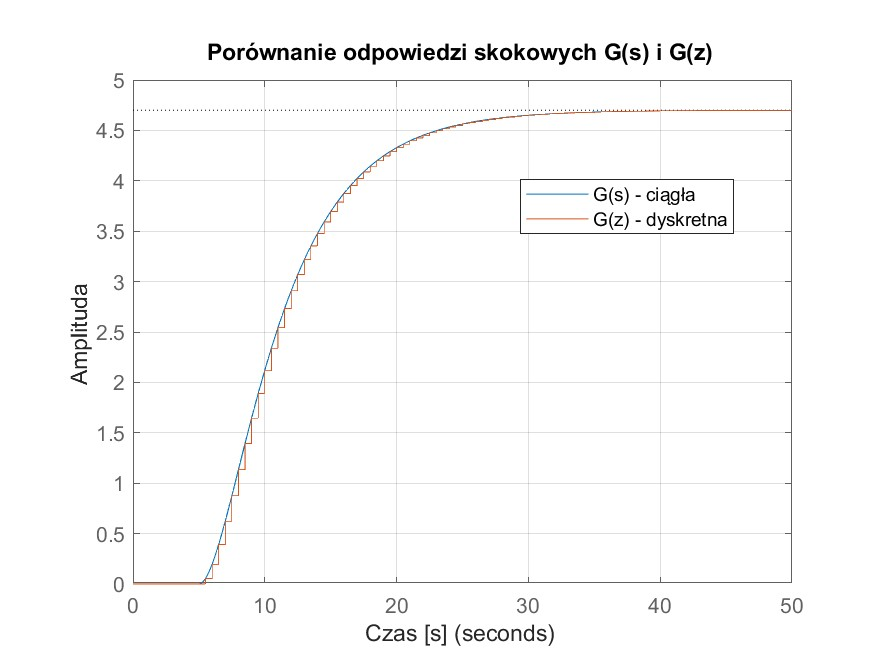
\includegraphics[width=0.8\textwidth]{pdf-modeli/zad1.pdf} % Użyj odpowiedniej ścieżki do pliku PDF
    \caption{Reprezentacja graficzna modelu obiektu w~Simulinku.}
    \label{rys:model_simulink}
\end{figure}

\FloatBarrier
\section{Weryfikacja modelu w~przestrzeni stanu}

Aby wykazać, że otrzymany model w~przestrzeni stanu jest poprawny, przekształcono go z~powrotem do postaci transmitancji za pomocą funkcji `ss2tf` w~MATLABie. Kod użyty do weryfikacji przedstawiono na listingu \ref{lst:ss2tf}.
\begin{lstlisting}[style=custommatlab, caption={Weryfikacja modelu w przestrzeni stanu.}, label={lst:ss2tf}]
[num_2, den_2] = ss2tf(A, B, C, D);
while length(num_2) > length(num) && abs(num_2(1)) < 1e-10
    num_2 = num_2(2:end);
end

if length(num_2) == length(num) && max(abs(num - num_2)) > 1e-10 || ...
   length(den_2) == length(den) && max(abs(den - den_2)) > 1e-10
    disp('Błąd przy konwersji na transmitancje');
end
\end{lstlisting}
Po konwersji i~ewentualnej normalizacji (usunięciu zer wiodących w~liczniku wynikających z~błędów numerycznych), otrzymano współczynniki licznika i~mianownika odpowiadające pierwotnej transmitancji (\ref{eq:transmitancja}). Potwierdza to poprawność wyznaczonego modelu w~przestrzeni stanu.

\FloatBarrier
\section{Regulator ze sprzężeniem od stanu}

Zaprojektowano regulator ze sprzężeniem od stanu postaci $u(t) = -Kx(t)$, gdzie $K$ jest wektorem wzmocnień. Celem regulatora jest stabilizacja obiektu i~sprowadzenie stanu do zera $x(t_{\text{konc}}) = [0, 0, 0, 0]^T$ z~warunku początkowego $x(0) = [-6, -3, -5, 1]^T$.

Wzmocnienia $K$ obliczono metodą lokowania biegunów za pomocą funkcji `acker` w~MATLABie. Założono, że wszystkie bieguny układu zamkniętego są rzeczywiste, takie same i~równe $s_b$. Przetestowano pięć wartości poczwórnego bieguna $s_b$: $\{-1, -2, -5, -7, -10\}$, odpowiadających konfiguracjom od ,,bardzo wolnej'' do ,,bardzo szybkiej''. Kod do obliczenia wzmocnień $K$ znajduje się na listingu \ref{lst:acker_K}.
\begin{lstlisting}[style=custommatlab, caption={Obliczenie wzmocnień regulatora K.}, label={lst:acker_K}]
sb = -2; % Przykładowa wartość bieguna
K = acker(A, B, [sb, sb, sb, sb]);
\end{lstlisting}
Symulacje przeprowadzono w~Simulinku, wykorzystując schemat przedstawiony na rys.~\ref{rys:regulator_simulink}. Czas symulacji $t_{\text{konc}}$ dobrano na $\SI{10}{\second}$, co okazało się wystarczające dla wszystkich konfiguracji.

\begin{figure}[H]
    \centering
    \includegraphics[width=0.9\textwidth]{pdf-modeli/zad3.pdf} % Użyj odpowiedniej ścieżki do pliku PDF
    \caption{Schemat blokowy układu z~regulatorem ze sprzężeniem od stanu w~Simulinku.}
    \label{rys:regulator_simulink}
\end{figure}

Wyniki symulacji dla różnych wartości $s_b$ przedstawiono na rysunkach \ref{rys:reg_x1} -- \ref{rys:reg_u}. Obliczono również wskaźniki jakości $J_x$ (całka z~sumy modułów zmiennych stanu) i~$J_u$ (rozpiętość sygnału sterującego), które zestawiono na rys.~\ref{rys:reg_metrics} oraz w~tabeli \ref{tab:reg_results}.

\begin{figure}[H]
    \centering
    \includegraphics[width=\textwidth]{plots/regulator_x1.jpg}
    \caption{Przebiegi zmiennej stanu $x_1(t)$ dla różnych wartości bieguna $s_b$.}
    \label{rys:reg_x1}
\end{figure}

\begin{figure}[H]
    \centering
    \includegraphics[width=\textwidth]{plots/regulator_x2.jpg}
    \caption{Przebiegi zmiennej stanu $x_2(t)$ dla różnych wartości bieguna $s_b$.}
    \label{rys:reg_x2}
\end{figure}

\begin{figure}[H]
    \centering
    \includegraphics[width=\textwidth]{plots/regulator_x3.jpg}
    \caption{Przebiegi zmiennej stanu $x_3(t)$ dla różnych wartości bieguna $s_b$.}
    \label{rys:reg_x3}
\end{figure}

\begin{figure}[H]
    \centering
    \includegraphics[width=\textwidth]{plots/regulator_x4.jpg}
    \caption{Przebiegi zmiennej stanu $x_4(t)$ dla różnych wartości bieguna $s_b$.}
    \label{rys:reg_x4}
\end{figure}

\begin{figure}[H]
    \centering
    \includegraphics[width=\textwidth]{plots/regulator_u.jpg}
    \caption{Przebiegi sygnału sterującego $u(t)$ dla różnych wartości bieguna $s_b$.}
    \label{rys:reg_u}
\end{figure}

\begin{figure}[H]
    \centering
    \includegraphics[width=0.7\textwidth]{plots/regulator_metrics.jpg}
    \caption{Wskaźniki jakości $J_x$ i~$J_u$ dla różnych wartości bieguna $s_b$.}
    \label{rys:reg_metrics}
\end{figure}

\begin{table}[H]
    \centering
    \caption{Zestawienie wskaźników jakości $J_x$ i $J_u$ dla różnych wartości bieguna $s_b$.}
    \label{tab:reg_results}
    \sisetup{table-number-alignment = center, table-text-alignment = center} % Ustawienia dla tej tabeli
    \begin{tabular}{|l|c|c|c|}
    \hline
    \input{plots/regulator_results.tex}
\end{table}

% Omówienie wyników i wybór regulatora
Z~przedstawionych przebiegów i~wskaźników jakości wynika, że im dalej w~lewo na osi rzeczywistej umieszczone są bieguny (większa wartość bezwzględna $s_b$), tym szybsza jest odpowiedź układu (szybsze dążenie zmiennych stanu do zera, mniejszy wskaźnik $J_x$). Jednakże, szybsza odpowiedź wiąże się z~większymi wartościami i~szybszymi zmianami sygnału sterującego $u(t)$, co odzwierciedla rosnący wskaźnik $J_u$.

Jako kompromis między szybkością regulacji a~jakością sygnału sterującego wybrano regulator z~biegunem $s_b = -2$. Zapewnia on stosunkowo szybkie osiągnięcie stanu równowagi przy akceptowalnym zakresie zmian sygnału sterującego. Dalsze symulacje będą prowadzone dla tej wartości $s_b$.

\FloatBarrier
\section{Obserwator stanu pełnego rzędu}

Zaprojektowano obserwator stanu pełnego rzędu w~celu estymacji wektora stanu $x(t)$. Równania obserwatora mają postać:
\begin{equation}
    \dot{\hat{x}}(t) = A\hat{x}(t) + Bu(t) + L(y(t) - \hat{y}(t))
    \label{eq:obs_rownanie_stanu}
\end{equation}
\begin{equation}
    \hat{y}(t) = C\hat{x}(t) + Du(t)
    \label{eq:obs_rownanie_wyjscia}
\end{equation}
gdzie $\hat{x}(t)$ jest wektorem estymowanego stanu, $\hat{y}(t)$ jest estymowanym wyjściem, a~$L$ jest macierzą (wektorem kolumnowym) wzmocnień obserwatora. Podstawiając macierze $A, B, C, D$, otrzymujemy szczegółowe równania (stosując obliczenia symboliczne matlab):

\begin{lstlisting}[style=custommatlab, caption={Obliczenie symboliczne równań obserwatora.}, label={lst:obs_eq}]
xhat = sym('xhat', [n 1]);
L = sym('L', [n 1]);


dxhat = A*xhat + B*u + L*(y - C*xhat - D*u);
yhat = C*xhat + D*u;
\end{lstlisting}

\begin{align}
    \dot{\hat{x}}_1(t) &= -12\hat{x}_1 - 29\hat{x}_2 + 102\hat{x}_3 + 360\hat{x}_4 + u - L_1(\hat{x}_3 + \hat{x}_4 - y) \nonumber \\
    \dot{\hat{x}}_2(t) &= \hat{x}_1 - L_2(\hat{x}_3 + \hat{x}_4 - y) \nonumber \\
    \dot{\hat{x}}_3(t) &= \hat{x}_2 - L_3(\hat{x}_3 + \hat{x}_4 - y) \label{eq:rownania_obserwatora} \\
    \dot{\hat{x}}_4(t) &= \hat{x}_3 - L_4(\hat{x}_3 + \hat{x}_4 - y) \nonumber
\end{align}
Estymowane wyjście:
\begin{equation}
    \hat{y}(t) = \hat{x}_3(t) + \hat{x}_4(t)
\end{equation}
Wzmocnienia $L$ obliczono metodą lokowania biegunów za pomocą funkcji `acker` w~MATLABie. Bieguny obserwatora $s_o$ umieszczono tak, aby dynamika błędu była szybsza niż dynamika układu zamkniętego z~regulatorem. % Wykorzystano dualność sterowania i~obserwacji, stosując funkcję `acker` do pary $(A^T, C^T)$ w~celu obliczenia $L^T$. Kod do obliczenia $L$ przedstawiono na listingu \ref{lst:acker_L}.
\begin{lstlisting}[style=custommatlab, caption={Obliczenie wzmocnień obserwatora L.}, label={lst:acker_L}]
so = -6;
L = acker(A', C', [so so so so]);
% Pominięto transpozycje w celu ułatwienia wykorzystania w Symulinku
\end{lstlisting}
Szczegółową strukturę obserwatora zaimplementowaną w~Simulinku przedstawiono na rys.~\ref{rys:obserwator_simulink}.

\begin{figure}[H]
    \centering
    \includegraphics[width=0.9\textwidth]{pdf-modeli/zad4.pdf} % Użyj odpowiedniej ścieżki do pliku PDF
    \caption{Szczegółowa struktura obserwatora stanu w~Simulinku.}
    \label{rys:obserwator_simulink}
\end{figure}

\FloatBarrier
\section{Testowanie obserwatora}

Działanie obserwatora przetestowano w~układzie zamkniętym z~wybranym wcześniej regulatorem ($s_b = -2$), który nadal korzystał z~rzeczywistego (mierzonego) stanu $x(t)$. Celem było sprawdzenie szybkości i~dokładności estymacji stanu przez obserwator dla różnych jego biegunów $s_o$. Schemat blokowy układu symulacyjnego przedstawiono na rys.~\ref{rys:test_obs_simulink}.

\begin{figure}[H]
    \centering
    \includegraphics[width=\textwidth]{pdf-modeli/zad5.pdf}
    \caption{Schemat blokowy układu do testowania obserwatora (regulator używa $x$).}
    \label{rys:test_obs_simulink}
\end{figure}

Symulacje przeprowadzono dla warunku początkowego obiektu $x(0) = [-6, -3, -5, 1]^T$ oraz zerowego warunku początkowego obserwatora $\hat{x}(0) = [0, 0, 0, 0]^T$. Przetestowano pięć wartości poczwórnego bieguna obserwatora $s_o$: $\{-3, -6, -15, -21, -30\}$. Czas symulacji wynosił $t_{\text{konc}} = \SI{10}{\second}$.

Na rysunkach \ref{rys:obs_err_x1} -- \ref{rys:obs_err_x4} przedstawiono przebiegi wartości bezwzględnych błędów estymacji $|x_i(t) - \hat{x}_i(t)|$ dla wszystkich testowanych biegunów $s_o$. Zastosowano skalę logarytmiczną na osi pionowej dla lepszej czytelności małych błędów. Obliczono również wskaźnik jakości estymacji $J_o$ (całka z~sumy modułów błędów estymacji), który zestawiono na rys.~\ref{rys:obs_metrics} oraz w~tabeli \ref{tab:obs_results}.

\begin{figure}[H]
    \centering
    \includegraphics[width=\textwidth]{plots/observer_x1_error.jpg}
    \caption{Przebiegi błędu estymacji $|x_1(t) - \hat{x}_1(t)|$ dla różnych wartości bieguna $s_o$.}
    \label{rys:obs_err_x1}
\end{figure}

\begin{figure}[H]
    \centering
    \includegraphics[width=\textwidth]{plots/observer_x2_error.jpg}
    \caption{Przebiegi błędu estymacji $|x_2(t) - \hat{x}_2(t)|$ dla różnych wartości bieguna $s_o$.}
    \label{rys:obs_err_x2}
\end{figure}

\begin{figure}[H]
    \centering
    \includegraphics[width=\textwidth]{plots/observer_x3_error.jpg}
    \caption{Przebiegi błędu estymacji $|x_3(t) - \hat{x}_3(t)|$ dla różnych wartości bieguna $s_o$.}
    \label{rys:obs_err_x3}
\end{figure}

\begin{figure}[H]
    \centering
    \includegraphics[width=\textwidth]{plots/observer_x4_error.jpg}
    \caption{Przebiegi błędu estymacji $|x_4(t) - \hat{x}_4(t)|$ dla różnych wartości bieguna $s_o$.}
    \label{rys:obs_err_x4}
\end{figure}

\begin{figure}[H]
    \centering
    \includegraphics[width=0.7\textwidth]{plots/observer_metrics.jpg}
    \caption{Wskaźnik jakości estymacji $J_o$ dla różnych wartości bieguna $s_o$.}
    \label{rys:obs_metrics}
\end{figure}

\begin{table}[H]
    \centering
    \caption{Zestawienie wskaźnika jakości estymacji $J_o$ dla różnych wartości bieguna $s_o$.}
    \label{tab:obs_results}
    \sisetup{table-number-alignment = center, table-text-alignment = center} % Ustawienia dla tej tabeli
    \begin{tabular}{|l|c|c|}
    \hline
    \input{plots/observer_results.tex}
\end{table}

% Omówienie wyników i wybór obserwatora
Z~przebiegów błędów estymacji oraz wskaźnika $J_o$ wynika, że im szybsze są bieguny obserwatora (większa wartość bezwzględna $s_o$), tym szybciej błąd estymacji dąży do zera i~mniejsza jest jego wartość całkowita ($J_o$). Obserwator z~biegunami $s_o = -30$ zapewnia najszybszą zbieżność estymaty do rzeczywistego stanu.

Wybrano obserwator z~biegunem $s_o = -6$ jako prezentujący najlepszy współczynnik $J_o$. Dalsze symulacje będą prowadzone dla tej wartości $s_o$.

\FloatBarrier
\section{Regulator z~obserwatorem}

Przetestowano działanie układu regulacji, w~którym regulator wykorzystuje stan estymowany przez obserwator, $\hat{x}(t)$, zamiast mierzonego stanu $x(t)$. Sygnał sterujący jest więc obliczany jako $u(t) = -K\hat{x}(t)$. Wykorzystano wybrany wcześniej regulator ($s_b = -2$) oraz wybrany obserwator ($s_o = -6$). Schemat blokowy układu symulacyjnego przedstawiono na rys.~\ref{rys:reg_obs_simulink}.

\begin{figure}[H]
    \centering
    \includegraphics[width=\textwidth]{pdf-modeli/zad6.pdf} % Użyj odpowiedniej ścieżki do pliku PDF
    \caption{Schemat blokowy układu z~regulatorem wykorzystującym stan obserwowany $\hat{x}$.}
    \label{rys:reg_obs_simulink}
\end{figure}

Symulacje przeprowadzono dla dwóch przypadków warunków początkowych obserwatora $\hat{x}(0)$:
\begin{enumerate}
    \item Zerowy warunek początkowy: $\hat{x}(0) = [0, 0, 0, 0]^T$
    \item Niezerowy warunek początkowy: $\hat{x}(0) = [-10, 10, -20, 20]^T$
\end{enumerate}
Warunek początkowy obiektu pozostał niezmieniony: $x(0) = [-6, -3, -5, 1]^T$. Czas symulacji wynosił $t_{\text{konc}} = \SI{10}{\second}$.

Przebiegi zmiennych stanu $x_i(t)$ oraz sygnału sterującego $u(t)$ dla obu przypadków warunków początkowych obserwatora przedstawiono na rysunkach \ref{rys:init_x1} -- \ref{rys:init_u}. Porównano również wskaźniki jakości $J_x$ i~$J_u$ (rys.~\ref{rys:init_metrics}, tab.~\ref{tab:init_results}).

\begin{figure}[H]
    \centering
    \includegraphics[width=\textwidth]{plots/init_cond_x1.jpg}
    \caption{Przebiegi zmiennej stanu $x_1(t)$ dla różnych warunków początkowych obserwatora.}
    \label{rys:init_x1}
\end{figure}

\begin{figure}[H]
    \centering
    \includegraphics[width=\textwidth]{plots/init_cond_x2.jpg}
    \caption{Przebiegi zmiennej stanu $x_2(t)$ dla różnych warunków początkowych obserwatora.}
    \label{rys:init_x2}
\end{figure}

\begin{figure}[H]
    \centering
    \includegraphics[width=\textwidth]{plots/init_cond_x3.jpg}
    \caption{Przebiegi zmiennej stanu $x_3(t)$ dla różnych warunków początkowych obserwatora.}
    \label{rys:init_x3}
\end{figure}

\begin{figure}[H]
    \centering
    \includegraphics[width=\textwidth]{plots/init_cond_x4.jpg}
    \caption{Przebiegi zmiennej stanu $x_4(t)$ dla różnych warunków początkowych obserwatora.}
    \label{rys:init_x4}
\end{figure}

\begin{figure}[H]
    \centering
    \includegraphics[width=\textwidth]{plots/init_cond_u.jpg}
    \caption{Przebiegi sygnału sterującego $u(t)$ dla różnych warunków początkowych obserwatora.}
    \label{rys:init_u}
\end{figure}

\begin{figure}[H]
    \centering
    \includegraphics[width=0.7\textwidth]{plots/init_cond_metrics.jpg}
    \caption{Wskaźniki jakości $J_x$ i~$J_u$ dla różnych warunków początkowych obserwatora.}
    \label{rys:init_metrics}
\end{figure}

\begin{table}[H]
    \centering
    \caption{Zestawienie wskaźników jakości $J_x$ i $J_u$ dla różnych warunków początkowych obserwatora.}
    \label{tab:init_results}
    \sisetup{table-number-alignment = center, table-text-alignment = center} % Ustawienia dla tej tabeli
    \begin{tabular}{|l| S[table-format = 3.4] | S[table-format = 5.4] |} % Definicja kolumn
        \hline
        \input{plots/init_cond_results.tex}
\end{table}

% Omówienie wyników
Porównując przebiegi dla zerowego i~niezerowego warunku początkowego obserwatora, można zauważyć, że w~przypadku niezerowego $\hat{x}(0)$ początkowa faza regulacji jest inna. Wynika to z~faktu, że regulator na początku działa w~oparciu o~błędną estymatę stanu. Jednak dzięki temu, że obserwator jest stabilny i~szybszy od regulatora ($s_o = -6$ vs $s_b = -2$), błąd estymacji szybko maleje, a~estymowany stan $\hat{x}(t)$ zbliża się do rzeczywistego stanu $x(t)$. Po pewnym czasie (ok. \SI{5}{\second}) przebiegi dla obu przypadków stabilizują się.

Niezerowy warunek początkowy obserwatora prowadzi do znacznie większych wartości wskaźników $J_x$ i~$J_u$, co jest spowodowane początkowym, mniej efektywnym sterowaniem. Mimo to, układ pozostaje stabilny i~osiąga stan równowagi. Potwierdza to poprawność działania zaprojektowanego układu regulacji z~obserwatorem.

\FloatBarrier
\chapter{Zadanie dodatkowe}

Zaprojektowano regulator ze sprzężeniem od stanu z~całkowaniem błędu regulacji. Celem jest zapewnienie zerowego błędu ustalonego w~zadaniu nadążania za wartością zadaną $y_{\text{zad}}(t)$ dla sygnału wyjściowego $y(t)$. Dla uproszczenia założono, że regulator korzysta z~mierzonego stanu $x(t)$.

Wprowadzono dodatkową zmienną stanu $x_e(t)$ (całka błędu):
\begin{equation}
    \dot{x}_e(t) = y_{\text{zad}}(t) - y(t) = y_{\text{zad}}(t) - Cx(t)
\end{equation}
Rozszerzony wektor stanu wynosi $x_{\text{aug}}(t) = [x(t)^T, x_e(t)]^T$. Równania stanu dla układu rozszerzonego mają postać:
\begin{equation}
    \dot{x}_{\text{aug}}(t) = A_e x_{\text{aug}}(t) + B_e u(t) + D_e y_{\text{zad}}(t)
\end{equation}
gdzie:
\begin{gather}
A_e = \begin{bmatrix} A & \boldsymbol{0}_{n \times 1} \\ -C & 0 \end{bmatrix} = \begin{bmatrix} -12 & -29 & 102 & 360 & 0 \\ 1 & 0 & 0 & 0 & 0 \\ 0 & 1 & 0 & 0 & 0 \\ 0 & 0 & 1 & 0 & 0 \\ 0 & 0 & -1 & -1 & 0 \end{bmatrix} \\
B_e = \begin{bmatrix} B \\ 0 \end{bmatrix} = \begin{bmatrix} 1 \\ 0 \\ 0 \\ 0 \\ 0 \end{bmatrix}, \quad
D_e = \begin{bmatrix} \boldsymbol{0}_{n \times 1} \\ 1 \end{bmatrix} = \begin{bmatrix} 0 \\ 0 \\ 0 \\ 0 \\ 1 \end{bmatrix}
\end{gather}
Sygnał sterujący jest postaci $u(t) = -K_e x_{\text{aug}}(t) = -[K, K_I] [x(t)^T, x_e(t)]^T$. Wzmocnienia $K_e = [K, K_I]$ obliczono metodą lokowania biegunów dla układu rozszerzonego $(A_e, B_e)$ za pomocą funkcji `acker`. Przetestowano trzy wartości pięciokrotnego bieguna $s_{b,e}$: $\{-2, -3.5, -5\}$ (,,wolny'', ,,średni'', ,,szybki''). Kod do obliczenia $K_e$ przedstawiono na listingu \ref{lst:acker_Ke}.
\begin{lstlisting}[style=custommatlab, caption={Obliczenie wzmocnień regulatora z całkowaniem Ke.}, label={lst:acker_Ke}]
sb_e = -2;
K_e = acker(A_e, B_e, [sb_e, sb_e, sb_e, sb_e, sb_e]);
\end{lstlisting}
Symulacje przeprowadzono w~Simulinku dla zadania nadążania za zmienną wartością zadaną $y_{\text{zad}}(t)$ (schodkową), przy zerowych warunkach początkowych obiektu $x_{\text{aug}}(0) = \boldsymbol{0}$. Schemat blokowy układu przedstawiono na rys.~\ref{rys:reg_int_simulink}. Czas symulacji wynosił $t_{\text{konc}} = \SI{20}{\second}$.

\begin{figure}[H]
    \centering
    \includegraphics[width=\textwidth]{pdf-modeli/zad_dod_1.pdf} % Użyj odpowiedniej ścieżki do pliku PDF
    \caption{Schemat blokowy układu z~regulatorem z~całkowaniem (korzystającym z $x$).}
    \label{rys:reg_int_simulink}
\end{figure}

\begin{figure}[H]
    \centering
    \includegraphics[width=\textwidth]{pdf-modeli/zad_dod_2.pdf} % Użyj odpowiedniej ścieżki do pliku PDF (lub tej samej co poprzednio, jeśli model jest ten sam)
    \caption{Schemat blokowy modelu z~całkowaniem.}
    \label{rys:reg_int_bmod_simulink}
\end{figure}

Przebiegi zmiennych stanu $x_1(t)$--$x_4(t)$, zmiennej całkującej $x_e(t)$, sygnału wyjściowego $y(t)$ na tle wartości zadanej $y_{\text{zad}}(t)$ oraz sygnału sterującego $u(t)$ dla trzech konfiguracji biegunów $s_{b,e}$ przedstawiono na rysunkach \ref{rys:int_x1} -- \ref{rys:int_u}.

\begin{figure}[H]
    \centering
    \includegraphics[width=\textwidth]{plots/int_regulator_x1.jpg}
    \caption{Przebiegi zmiennej stanu $x_1(t)$ dla regulatora z~całkowaniem (nominalny B).}
    \label{rys:int_x1}
\end{figure}

\begin{figure}[H]
    \centering
    \includegraphics[width=\textwidth]{plots/int_regulator_x2.jpg}
    \caption{Przebiegi zmiennej stanu $x_2(t)$ dla regulatora z~całkowaniem (nominalny B).}
    \label{rys:int_x2}
\end{figure}

\begin{figure}[H]
    \centering
    \includegraphics[width=\textwidth]{plots/int_regulator_x3.jpg}
    \caption{Przebiegi zmiennej stanu $x_3(t)$ dla regulatora z~całkowaniem (nominalny B).}
    \label{rys:int_x3}
\end{figure}

\begin{figure}[H]
    \centering
    \includegraphics[width=\textwidth]{plots/int_regulator_x4.jpg}
    \caption{Przebiegi zmiennej stanu $x_4(t)$ dla regulatora z~całkowaniem (nominalny B).}
    \label{rys:int_x4}
\end{figure}

\begin{figure}[H]
    \centering
    \includegraphics[width=\textwidth]{plots/int_regulator_xe.jpg}
    \caption{Przebiegi zmiennej całkującej $x_e(t)$ dla regulatora z~całkowaniem (nominalny B).}
    \label{rys:int_xe}
\end{figure}

\begin{figure}[H]
    \centering
    \includegraphics[width=\textwidth]{plots/int_regulator_y.jpg}
    \caption{Przebiegi wyjścia $y(t)$ i~wartości zadanej $y_{zad}(t)$ dla regulatora z~całkowaniem (nominalny B).}
    \label{rys:int_y}
\end{figure}

\begin{figure}[H]
    \centering
    \includegraphics[width=\textwidth]{plots/int_regulator_u.jpg}
    \caption{Przebiegi sygnału sterującego $u(t)$ dla regulatora z~całkowaniem (nominalny B).}
    \label{rys:int_u}
\end{figure}

% Omówienie wyników nominalnych
Jak oczekiwano, regulator z~całkowaniem zapewnia zerowy błąd ustalony ($y(t) \to y_{\text{zad}}(t)$) dla stałych wartości zadanych. Szybkość odpowiedzi zależy od położenia biegunów $s_{b,e}$ -- im dalej w~lewo, tym szybsze jest nadążanie za zmianami $y_{\text{zad}}(t)$, ale wiąże się to z~większymi wartościami sygnału sterującego $u(t)$ w~stanach przejściowych oraz większym przesterowaniem.

\FloatBarrier
\subsection*{Test odporności na błąd modelowania}

Przeprowadzono dodatkowe symulacje w~celu sprawdzenia odporności regulatora z~całkowaniem na błąd modelowania. W~symulacji obiektu zwiększono wartość wszystkich elementów macierzy $B$ o~30\% ($B_{\text{rzecz}} = 1.3 \times B$), podczas gdy regulator nadal był zaprojektowany dla nominalnej macierzy $B$. Schemat symulacyjny pozostał ten sam (rys.~\ref{rys:reg_int_simulink}, ewentualnie rys.~\ref{rys:reg_int_bmod_simulink} jeśli był dedykowany), zmieniono jedynie parametry bloku obiektu.

Wyniki symulacji dla przypadku ze zmienioną macierzą $B$ przedstawiono na rysunkach \ref{rys:int_bmod_x1} -- \ref{rys:int_bmod_u}.

\begin{figure}[H]
    \centering
    \includegraphics[width=\textwidth]{plots/int_regulator_x1_Bmod.jpg}
    \caption{Przebiegi zmiennej stanu $x_1(t)$ dla regulatora z~całkowaniem (B obiektu +30\%).}
    \label{rys:int_bmod_x1}
\end{figure}

\begin{figure}[H]
    \centering
    \includegraphics[width=\textwidth]{plots/int_regulator_x2_Bmod.jpg}
    \caption{Przebiegi zmiennej stanu $x_2(t)$ dla regulatora z~całkowaniem (B obiektu +30\%).}
    \label{rys:int_bmod_x2}
\end{figure}

\begin{figure}[H]
    \centering
    \includegraphics[width=\textwidth]{plots/int_regulator_x3_Bmod.jpg}
    \caption{Przebiegi zmiennej stanu $x_3(t)$ dla regulatora z~całkowaniem (B obiektu +30\%).}
    \label{rys:int_bmod_x3}
\end{figure}

\begin{figure}[H]
    \centering
    \includegraphics[width=\textwidth]{plots/int_regulator_x4_Bmod.jpg}
    \caption{Przebiegi zmiennej stanu $x_4(t)$ dla regulatora z~całkowaniem (B obiektu +30\%).}
    \label{rys:int_bmod_x4}
\end{figure}

\begin{figure}[H]
    \centering
    \includegraphics[width=\textwidth]{plots/int_regulator_xe_Bmod.jpg}
    \caption{Przebiegi zmiennej całkującej $x_e(t)$ dla regulatora z~całkowaniem (B obiektu +30\%).}
    \label{rys:int_bmod_xe}
\end{figure}

\begin{figure}[H]
    \centering
    \includegraphics[width=\textwidth]{plots/int_regulator_y_Bmod.jpg}
    \caption{Przebiegi wyjścia $y(t)$ i~wartości zadanej $y_{zad}(t)$ dla regulatora z~całkowaniem (B obiektu +30\%).}
    \label{rys:int_bmod_y}
\end{figure}

\begin{figure}[H]
    \centering
    \includegraphics[width=\textwidth]{plots/int_regulator_u_Bmod.jpg}
    \caption{Przebiegi sygnału sterującego $u(t)$ dla regulatora z~całkowaniem (B obiektu +30\%).}
    \label{rys:int_bmod_u}
\end{figure}

% Omówienie wyników z błędem modelowania
Porównując wyniki z~przypadkiem nominalnym (rys.~\ref{rys:int_x1} -- \ref{rys:int_u}), widać, że błąd modelowania (niedopasowanie wzmocnienia obiektu) wpływa na dynamikę odpowiedzi układu. Odpowiedzi są bardziej przesterowane i~bardziej oscylacyjne. Jest to zgodne z~oczekiwaniami, ponieważ rzeczywisty obiekt ma większe wzmocnienie niż zakładał regulator. Co ciekawe czym bieguny szybsze regulatora tym odporność na niedokładność modelowania większa.

% Co najważniejsze, dzięki działaniu całkującemu, regulator nadal zapewnia zerowy błąd ustalony ($y(t) \to y_{\text{zad}}(t)$) pomimo błędu modelowania. Potwierdza to podstawową zaletę wprowadzania członu całkującego – zwiększenie odporności układu regulacji na stałe zakłócenia i~błędy modelowania w~odniesieniu do błędu ustalonego.

\FloatBarrier
\chapter{Kody źródłowe} \label{chap:kody}

W~tej części zamieszczono pełne kody źródłowe skryptów MATLAB wykorzystanych do realizacji projektu. Modele Simulink (\texttt{model1.slx}, \texttt{model2.slx}, \texttt{model3.slx}) zostały dostarczone w formie pliku.

\section{equasions.m}

Listing \ref{lst:equasions_full} przedstawia pełny kod skryptu \texttt{equasions.m}, użyty do wyznaczenia macierzy stanu, weryfikacji oraz symbolicznego wyprowadzenia równań stanu, obserwatora i~układu rozszerzonego.

\begin{lstlisting}[style=custommatlab, caption={Pełny kod skryptu \texttt{equasions.m}.}, label={lst:equasions_full}]
%% Definicja transmitancji symbolicznej i konwersja na postać stanu
syms s u y xe yzad;
G = (s + 1) / ((s - 3) * (s + 4) * (s + 5) * (s + 6));

[num, den] = numden(G);
num = sym2poly(num);
den = sym2poly(den);

%% Zadanie 1

[A, B, C, D] = tf2ss(num, den);
n = size(A,1);

%% Zadanie 2
[num_2, den_2] = ss2tf(A, B, C, D);
while length(num_2) > length(num) && abs(num_2(1)) < 1e-10
    num_2 = num_2(2:end);
end

if length(num_2) == length(num) && max(abs(num - num_2)) > 1e-10 || ...
    length(den_2) == length(den) && max(abs(den - den_2)) > 1e-10
    disp('Błąd przy konwersji na transmitancje');
end

%% Inicjalizacja zmiennych symbolicznych

A_e = [A, zeros(n,1); -C, 0];
B_e = [B; 0];
n_e = size(A_e,1);


x = sym('x', [n 1]);
x_e = [x; xe];

xhat = sym('xhat', [n 1]);
L = sym('L', [n 1]);


%% Obliczenie równań symbolicznych
dx = A*x + B*u;
yr = C*x + D*u;

dxhat = A*xhat + B*u + L*(y - C*xhat - D*u);
yhat = C*xhat + D*u;

dxi = A_e*x_e + B_e*u + [zeros(4,1); 1]*yzad;

%% Równania regulatora

disp(' ');
disp('Równania stanu:');
for i = 1:n
    disp(['dx', num2str(i), '/dt = ', char(dx(i))]);
end

disp(' ');
disp('Równanie wyjścia:');
disp(['y = ', char(yr)]);

%% Równania obserwatora
disp(' ');
disp('Równania obserwatora:');
for i = 1:n
    disp(['dxhat', num2str(i), '/dt = ', char(dxhat(i))]);
end

disp(' ');
disp('Równanie wyjścia obserwatora:');
disp(['yhat = ', char(yhat)]);

%% Równania regulatora z całkowaniem
disp(' ');
disp('Równania dla regulatora z całkowaniem:');

for i = 1:n
    disp(['dx', num2str(i), '/dt = ', char(dxi(i))]);
end
disp(['dxe/dt = ', char(dxi(n_e))]);

disp(' ');
disp('Równanie wyjścia:');
disp(['y = ', char(yr)]);

clear;
\end{lstlisting}

\section{data\_initialization.m}

Listing \ref{lst:init_full} pokazuje pełny kod skryptu \texttt{data\_initialization.m}, który inicjalizuje parametry symulacji (macierze stanu, warunki początkowe, wartości zadane) oraz oblicza wzmocnienia regulatorów ($K, K_e$) i~obserwatora ($L$) za pomocą funkcji `acker` dla wybranych (przykładowych) wartości biegunów.

\begin{lstlisting}[style=custommatlab, caption={Pełny kod skryptu \texttt{initializasja\_danych.m}.}, label={lst:init_full}]
syms s;
G = (s + 1) / ((s - 3) * (s + 4) * (s + 5) * (s + 6));

[num, den] = numden(G);
num = sym2poly(num);
den = sym2poly(den);
clear G s;

[A, B, C, D] = tf2ss(num, den);

A_e = [A, zeros(4,1); -C, 0];
B_e = [B; 0];

sb = -2;
so = -6;
sb_e = -2;

K = acker(A, B, [sb, sb, sb, sb]);
K_e = acker(A_e, B_e, [sb_e, sb_e, sb_e, sb_e, sb_e]);
L = acker(A', C', [so so so so]);

x0_m = [-6 -3 -5 1];
x0_r = [0 0 0 0 0];
x0_o = [0 0 0 0];

yzad = timeseries([-10, 10], [0, 10]);

clear A B C A_e B_e sb so sb_e;
\end{lstlisting}

\section{\texttt{combined\_plots.m}}

Skrypt \texttt{combined\_plots.m} jest odpowiedzialny za przeprowadzenie wszystkich symulacji opisanych w~rozdziałach 2 i~3 (zadania \texttt{3, 5, 6, dodatkowe}) oraz za wygenerowanie odpowiadających im wykresów i~tabel z~wynikami.
Skrypt ten automatyzuje proces testowania różnych konfiguracji i~prezentacji wyników w~jednolity sposób, zgodnie z~wymaganiami projektu.

\begin{lstlisting}[style=custommatlab, caption={Pełny kod skryptu \texttt{combined\_plots.m}.}, label={lst:init_full}]
output_dir = '../plots';

if ~exist(output_dir, 'dir')
    mkdir(output_dir);
end

% Nazwy plików wyjściowych
filenames = struct(...
    'regulator_x1', 'regulator_x1.jpg', ...
    'regulator_x2', 'regulator_x2.jpg', ...
    'regulator_x3', 'regulator_x3.jpg', ...
    'regulator_x4', 'regulator_x4.jpg', ...
    'regulator_u', 'regulator_u.jpg', ...
    'regulator_metrics', 'regulator_metrics.jpg', ...
    'observer_x1_error', 'observer_x1_error.jpg', ...
    'observer_x2_error', 'observer_x2_error.jpg', ...
    'observer_x3_error', 'observer_x3_error.jpg', ...
    'observer_x4_error', 'observer_x4_error.jpg', ...
    'observer_metrics', 'observer_metrics.jpg', ...
    'init_cond_x1', 'init_cond_x1.jpg', ...
    'init_cond_x2', 'init_cond_x2.jpg', ...
    'init_cond_x3', 'init_cond_x3.jpg', ...
    'init_cond_x4', 'init_cond_x4.jpg', ...
    'init_cond_u', 'init_cond_u.jpg', ...
    'init_cond_metrics', 'init_cond_metrics.jpg', ...
    'regulator_table', 'regulator_results.tex', ...
    'observer_table', 'observer_results.tex', ...
    'init_cond_table', 'init_cond_results.tex', ...
    'int_regulator_x1', 'int_regulator_x1.jpg', ...
    'int_regulator_x2', 'int_regulator_x2.jpg', ...
    'int_regulator_x3', 'int_regulator_x3.jpg', ...
    'int_regulator_x4', 'int_regulator_x4.jpg', ...
    'int_regulator_xe', 'int_regulator_xe.jpg', ...
    'int_regulator_y', 'int_regulator_y.jpg', ...
    'int_regulator_u', 'int_regulator_u.jpg', ...
    'int_regulator_x1_Bmod', 'int_regulator_x1_Bmod.jpg', ...
    'int_regulator_x2_Bmod', 'int_regulator_x2_Bmod.jpg', ...
    'int_regulator_x3_Bmod', 'int_regulator_x3_Bmod.jpg', ...
    'int_regulator_x4_Bmod', 'int_regulator_x4_Bmod.jpg', ...
    'int_regulator_xe_Bmod', 'int_regulator_xe_Bmod.jpg', ...
    'int_regulator_y_Bmod', 'int_regulator_y_Bmod.jpg', ...
    'int_regulator_u_Bmod', 'int_regulator_u_Bmod.jpg');

%% Zadanie 3

pole_configs = {'bardzo\_wolny', 'wolny', 'średni', 'szybki', 'bardzo\_szybki'};
pole_configs_raw = {'bardzo_wolny', 'wolny', 'średni', 'szybki', 'bardzo_szybki'};
sb_values = [-1, -2, -5, -7, -10];
t_end = 10;
x0_m = [-6 -3 -5 1];
x0_o = [0 0 0 0];

time_data_reg = cell(length(pole_configs), 1);
x1_reg = cell(length(pole_configs), 1);
x2_reg = cell(length(pole_configs), 1);
x3_reg = cell(length(pole_configs), 1);
x4_reg = cell(length(pole_configs), 1);
u_reg = cell(length(pole_configs), 1);
Jx_reg = zeros(1, length(pole_configs));
Ju_reg = zeros(1, length(pole_configs));

for i = 1:length(pole_configs)
    K = acker(A, B, [sb_values(i), sb_values(i), sb_values(i), sb_values(i)]);
    out = sim('model1.slx', 'StopTime', num2str(t_end));
    time_data_reg{i} = out.x1_data.Time;
    x1_reg{i} = out.x1_data.Data;
    x2_reg{i} = out.x2_data.Data;
    x3_reg{i} = out.x3_data.Data;
    x4_reg{i} = out.x4_data.Data;
    u_reg{i} = out.u_data.Data;
    Jx_reg(i) = out.Jx_data.Data(end);
    Ju_reg(i) = out.Ju_data.Data(end);
    fprintf('Test Regulatora %d/%d: %s (sb = %.1f)\n', i, ...
        length(pole_configs), pole_configs_raw{i}, sb_values(i));
end

%% Zadanie 5

observer_configs = {'bardzo\_wolny', 'wolny', 'średni', 'szybki', 'bardzo\_szybki'};
observer_configs_raw = {'bardzo_wolny', 'wolny', 'średni', 'szybki', 'bardzo_szybki'};
so_values = [-3, -6, -15, -21, -30];
sb = -2;
K = acker(A, B, [sb, sb, sb, sb]);

time_data_obs = cell(length(observer_configs), 1);
x1_diff = cell(length(observer_configs), 1);
x2_diff = cell(length(observer_configs), 1);
x3_diff = cell(length(observer_configs), 1);
x4_diff = cell(length(observer_configs), 1);
Jo = zeros(1, length(observer_configs));

for i = 1:length(observer_configs)
    L = acker(A', C', [so_values(i), so_values(i), so_values(i), so_values(i)])';
    out = sim('model1.slx', 'StopTime', num2str(t_end));
    time_data_obs{i} = out.x1_o_data.Time;
    x1_diff{i} = out.x1_o_data.Data;
    x2_diff{i} = out.x2_o_data.Data;
    x3_diff{i} = out.x3_o_data.Data;
    x4_diff{i} = out.x4_o_data.Data;
    Jo(i) = out.Jo_data.Data(end);
    fprintf('Test Obserwatora %d/%d: %s (so = %.1f)\n', i, ...
        length(observer_configs), observer_configs_raw{i}, so_values(i));
end

%% Zadanie 6

sb = -2;
so = -6;
K = acker(A, B, [sb, sb, sb, sb]);
L = acker(A', C', [so, so, so, so])';

observer_cases = {'Zerowy\_warunek\_początkowy', 'Niezerowy\_warunek\_początkowy'};
observer_cases_raw = {'Zerowy_warunek_początkowy', 'Niezerowy_warunek_początkowy'};
x0_m = [-6, -3, -5, 1];
x0_o_tested = [0, 0, 0, 0; -10, 10, -20, 20];

time_data_init = cell(2, 1);
x1_init = cell(2, 1);
x2_init = cell(2, 1);
x3_init = cell(2, 1);
x4_init = cell(2, 1);
u_init = cell(2, 1);
Jx_init = zeros(1, 2);
Ju_init = zeros(1, 2);

for i = 1:length(observer_cases)
    x0_o = x0_o_tested(i, :);
    out = sim('model2.slx', 'StopTime', num2str(t_end));
    time_data_init{i} = out.x1_data.Time;
    x1_init{i} = out.x1_data.Data;
    x2_init{i} = out.x2_data.Data;
    x3_init{i} = out.x3_data.Data;
    x4_init{i} = out.x4_data.Data;
    u_init{i} = out.u_data.Data;
    Jx_init(i) = out.Jx_data.Data(end);
    Ju_init(i) = out.Ju_data.Data(end);
    fprintf('Test warunku początkowego %d/2: %s\n', i, observer_cases_raw{i});
end

%% Zadanie dodatkowe

int_configs = {'wolny', 'średni', 'szybki'};
int_configs_tex = {'wolny', 'średni', 'szybki'};
sb_int_values = [-2, -3.5, -5];

A_e = [A, zeros(size(A,1),1); -C, 0];
B_e = [B; 0];

t_end_int = 20;
x0_aug = zeros(size(A_e,1),1);

yzad_time = [0 5 10 15];
yzad_values = [-0.5 1 -1 0.5];

time_data_int = cell(length(int_configs), 1);
x1_int = cell(length(int_configs), 1);
x2_int = cell(length(int_configs), 1);
x3_int = cell(length(int_configs), 1);
x4_int = cell(length(int_configs), 1);
xe_int = cell(length(int_configs), 1);
y_set_int = cell(length(int_configs), 1);
y_int = cell(length(int_configs), 1);
u_int = cell(length(int_configs), 1);

for i = 1:length(int_configs)
    K_e = acker(A_e, B_e, [repmat(sb_int_values(i),1,5)]);

    yzad = timeseries(yzad_values, yzad_time);

    out = sim('model3.slx', 'StopTime', num2str(t_end_int));

    time_data_int{i} = out.x1_data.Time;
    x1_int{i} = out.x1_data.Data;
    x2_int{i} = out.x2_data.Data;
    x3_int{i} = out.x3_data.Data;
    x4_int{i} = out.x4_data.Data;
    xe_int{i} = out.xe_data.Data;
    y_set_int{i} = yzad.Data;
    y_int{i} = out.y_data.Data;
    u_int{i} = out.u_data.Data;

    fprintf('Test regulatora z całkowaniem %d/%d: %s (sb = %.1f)\n', ...
        i, length(int_configs), int_configs{i}, sb_int_values(i));
end

B_e_mod = [B*1.3; 0];
time_data_int_mod = cell(length(int_configs), 1);
x1_int_mod = cell(length(int_configs), 1);
x2_int_mod = cell(length(int_configs), 1);
x3_int_mod = cell(length(int_configs), 1);
x4_int_mod = cell(length(int_configs), 1);
xe_int_mod = cell(length(int_configs), 1);
y_set_int_mod = cell(length(int_configs), 1);
y_int_mod = cell(length(int_configs), 1);
u_int_mod = cell(length(int_configs), 1);

for i = 1:length(int_configs)
    K_e = acker(A_e, B_e_mod, [repmat(sb_int_values(i),1,5)]);

    yzad = timeseries(yzad_values, yzad_time);

    out = sim('model3.slx', 'StopTime', num2str(t_end_int));

    time_data_int_mod{i} = out.x1_data.Time;
    x1_int_mod{i} = out.x1_data.Data;
    x2_int_mod{i} = out.x2_data.Data;
    x3_int_mod{i} = out.x3_data.Data;
    x4_int_mod{i} = out.x4_data.Data;
    xe_int_mod{i} = out.xe_data.Data;
    y_set_int_mod{i} = yzad.Data;
    y_int_mod{i} = out.y_data.Data;
    u_int_mod{i} = out.u_data.Data;

    fprintf('Test regulatora z całkowaniem (B+30%%) %d/%d: %s (sb = %.1f)\n', ...
        i, length(int_configs), int_configs{i}, sb_int_values(i));
end

%% Tworzenie i zapisywanie wykresów

lineStyles = {'-', '--', ':', '-.', '-'};
figure_size = [0, 0, 1200, 800];

% Zadanie 3
fig = figure('Visible', 'off', 'Position', figure_size);
for i = 1:length(pole_configs)
    plot(time_data_reg{i}, x1_reg{i}, lineStyles{i}, 'LineWidth', 1.5);
    hold on;
end
title('Zmienna stanu x_1');
xlabel('Czas (s)'); ylabel('x_1');
legend(pole_configs, 'Location', 'best', 'Interpreter', 'tex');
grid on;
saveas(fig, fullfile(output_dir, filenames.regulator_x1));
close(fig);

fig = figure('Visible', 'off', 'Position', figure_size);
for i = 1:length(pole_configs)
    plot(time_data_reg{i}, x2_reg{i}, lineStyles{i}, 'LineWidth', 1.5);
    hold on;
end
title('Zmienna stanu x_2');
xlabel('Czas (s)'); ylabel('x_2');
legend(pole_configs, 'Location', 'best', 'Interpreter', 'tex');
grid on;
saveas(fig, fullfile(output_dir, filenames.regulator_x2));
close(fig);

fig = figure('Visible', 'off', 'Position', figure_size);
for i = 1:length(pole_configs)
    plot(time_data_reg{i}, x3_reg{i}, lineStyles{i}, 'LineWidth', 1.5);
    hold on;
end
title('Zmienna stanu x_3');
xlabel('Czas (s)'); ylabel('x_3');
legend(pole_configs, 'Location', 'best', 'Interpreter', 'tex');
grid on;
saveas(fig, fullfile(output_dir, filenames.regulator_x3));
close(fig);

fig = figure('Visible', 'off', 'Position', figure_size);
for i = 1:length(pole_configs)
    plot(time_data_reg{i}, x4_reg{i}, lineStyles{i}, 'LineWidth', 1.5);
    hold on;
end
title('Zmienna stanu x_4');
xlabel('Czas (s)'); ylabel('x_4');
legend(pole_configs, 'Location', 'best', 'Interpreter', 'tex');
grid on;
saveas(fig, fullfile(output_dir, filenames.regulator_x4));
close(fig);

fig = figure('Visible', 'off', 'Position', figure_size);
for i = 1:length(pole_configs)
    plot(time_data_reg{i}, u_reg{i}, lineStyles{i}, 'LineWidth', 1.5);
    hold on;
end
title('Sygnał sterujący u(t)');
xlabel('Czas (s)'); ylabel('u');
legend(pole_configs, 'Location', 'best', 'Interpreter', 'tex');
grid on;
saveas(fig, fullfile(output_dir, filenames.regulator_u));
close(fig);

% Wykres Ju i Jx
fig = figure('Visible', 'off', 'Position', figure_size);
x_categories = categorical(pole_configs);
x_categories = reordercats(x_categories, pole_configs);

yyaxis left
b1 = bar(x_categories, Jx_reg, 'FaceColor', 'blue');
ylabel('J_x');
ax = gca;
ax.YColor = 'blue';
hold on;

yyaxis right
b2 = bar(x_categories, Ju_reg, 'FaceColor', 'red', 'FaceAlpha', 0.6);
ylabel('J_u');
ax = gca;
ax.YColor = 'red';
hold off;

title('Metryki wydajności');
xlabel('Konfiguracja biegunów');
set(gca, 'XTickLabel', pole_configs, 'TickLabelInterpreter', 'tex');
legend([b1, b2], 'J_x', 'J_u', 'Location', 'best');
grid on;
saveas(fig, fullfile(output_dir, filenames.regulator_metrics));
close(fig);

% Zadanie 5
fig = figure('Visible', 'off', 'Position', figure_size);
for i = 1:length(observer_configs)
    semilogy(time_data_obs{i}, x1_diff{i}, lineStyles{i}, 'LineWidth', 1.5);
    hold on;
end
title('Błąd estymacji stanu |x_1 - x_1\_hat|');
xlabel('Czas (s)'); ylabel('|x_1 - x_1\_hat|');
legend(observer_configs, 'Location', 'best', 'Interpreter', 'tex');
grid on;
saveas(fig, fullfile(output_dir, filenames.observer_x1_error));
close(fig);

fig = figure('Visible', 'off', 'Position', figure_size);
for i = 1:length(observer_configs)
    semilogy(time_data_obs{i}, x2_diff{i}, lineStyles{i}, 'LineWidth', 1.5);
    hold on;
end
title('Błąd estymacji stanu |x_2 - x_2\_hat|');
xlabel('Czas (s)'); ylabel('|x_2 - x_2\_hat|');
legend(observer_configs, 'Location', 'best', 'Interpreter', 'tex');
grid on;
saveas(fig, fullfile(output_dir, filenames.observer_x2_error));
close(fig);

fig = figure('Visible', 'off', 'Position', figure_size);
for i = 1:length(observer_configs)
    semilogy(time_data_obs{i}, x3_diff{i}, lineStyles{i}, 'LineWidth', 1.5);
    hold on;
end
title('Błąd estymacji stanu |x_3 - x_3\_hat|');
xlabel('Czas (s)'); ylabel('|x_3 - x_3\_hat|');
legend(observer_configs, 'Location', 'best', 'Interpreter', 'tex');
grid on;
saveas(fig, fullfile(output_dir, filenames.observer_x3_error));
close(fig);

fig = figure('Visible', 'off', 'Position', figure_size);
for i = 1:length(observer_configs)
    semilogy(time_data_obs{i}, x4_diff{i}, lineStyles{i}, 'LineWidth', 1.5);
    hold on;
end
title('Błąd estymacji stanu |x_4 - x_4\_hat|');
xlabel('Czas (s)'); ylabel('|x_4 - x_4\_hat|');
legend(observer_configs, 'Location', 'best', 'Interpreter', 'tex');
grid on;
saveas(fig, fullfile(output_dir, filenames.observer_x4_error));
close(fig);

fig = figure('Visible', 'off', 'Position', figure_size);
bar(Jo);
title('Metryka wydajności obserwatora J_o');
xlabel('Konfiguracja biegunów');
set(gca, 'XTickLabel', observer_configs, 'TickLabelInterpreter', 'tex');
ylabel('J_o');
grid on;
saveas(fig, fullfile(output_dir, filenames.observer_metrics));
close(fig);

%% Zadanie 6
fig = figure('Visible', 'off', 'Position', figure_size);
for i = 1:length(observer_cases)
    plot(time_data_init{i}, x1_init{i}, lineStyles{i}, 'LineWidth', 1.5);
    hold on;
end
title('Zmienna stanu x_1');
xlabel('Czas (s)'); ylabel('x_1');
legend(observer_cases, 'Location', 'best', 'Interpreter', 'tex');
grid on;
saveas(fig, fullfile(output_dir, filenames.init_cond_x1));
close(fig);

fig = figure('Visible', 'off', 'Position', figure_size);
for i = 1:length(observer_cases)
    plot(time_data_init{i}, x2_init{i}, lineStyles{i}, 'LineWidth', 1.5);
    hold on;
end
title('Zmienna stanu x_2');
xlabel('Czas (s)'); ylabel('x_2');
legend(observer_cases, 'Location', 'best', 'Interpreter', 'tex');
grid on;
saveas(fig, fullfile(output_dir, filenames.init_cond_x2));
close(fig);

fig = figure('Visible', 'off', 'Position', figure_size);
for i = 1:length(observer_cases)
    plot(time_data_init{i}, x3_init{i}, lineStyles{i}, 'LineWidth', 1.5);
    hold on;
end
title('Zmienna stanu x_3');
xlabel('Czas (s)'); ylabel('x_3');
legend(observer_cases, 'Location', 'best', 'Interpreter', 'tex');
grid on;
saveas(fig, fullfile(output_dir, filenames.init_cond_x3));
close(fig);

fig = figure('Visible', 'off', 'Position', figure_size);
for i = 1:length(observer_cases)
    plot(time_data_init{i}, x4_init{i}, lineStyles{i}, 'LineWidth', 1.5);
    hold on;
end
title('Zmienna stanu x_4');
xlabel('Czas (s)'); ylabel('x_4');
legend(observer_cases, 'Location', 'best', 'Interpreter', 'tex');
grid on;
saveas(fig, fullfile(output_dir, filenames.init_cond_x4));
close(fig);

fig = figure('Visible', 'off', 'Position', figure_size);
for i = 1:length(observer_cases)
    plot(time_data_init{i}, u_init{i}, lineStyles{i}, 'LineWidth', 1.5);
    hold on;
end
title('Sygnał sterujący u(t)');
xlabel('Czas (s)'); ylabel('u');
legend(observer_cases, 'Location', 'best', 'Interpreter', 'tex');
grid on;
saveas(fig, fullfile(output_dir, filenames.init_cond_u));
close(fig);

% Wykres Ju i Jx
fig = figure('Visible', 'off', 'Position', figure_size);
x_categories_init = categorical(observer_cases);
x_categories_init = reordercats(x_categories_init, observer_cases);

yyaxis left
b1_init = bar(x_categories_init, Jx_init, 'FaceColor', 'blue');
ylabel('J_x');
ax = gca;
ax.YColor = 'blue';
hold on;

yyaxis right
b2_init = bar(x_categories_init, Ju_init, 'FaceColor', 'red', 'FaceAlpha', 0.6);
ylabel('J_u');
ax = gca;
ax.YColor = 'red';
hold off;

title('Ju i Jx');
xlabel('Warunek początkowy obserwatora');
set(gca, 'XTickLabel', observer_cases, 'TickLabelInterpreter', 'tex');
legend([b1_init, b2_init], 'J_x', 'J_u', 'Location', 'best');
grid on;
saveas(fig, fullfile(output_dir, filenames.init_cond_metrics));
close(fig);


%% Zadanie dodatkowe (nominalne B)

fig = figure('Visible', 'off', 'Position', figure_size);
hold on;
for i = 1:length(int_configs)
    plot(time_data_int{i}, x1_int{i}, lineStyles{i}, 'LineWidth', 1.5);
end
title('x_1(t) dla wszystkich biegunów');
xlabel('Czas (s)');
ylabel('x_1');
legend(int_configs_tex, 'Location', 'best', 'Interpreter', 'tex');
grid on;
saveas(fig, fullfile(output_dir, filenames.int_regulator_x1));
close(fig);

fig = figure('Visible', 'off', 'Position', figure_size);
hold on;
for i = 1:length(int_configs)
    plot(time_data_int{i}, x2_int{i}, lineStyles{i}, 'LineWidth', 1.5);
end
title('x_2(t) dla wszystkich biegunów');
xlabel('Czas (s)');
ylabel('x_2');
legend(int_configs_tex, 'Location', 'best', 'Interpreter', 'tex');
grid on;
saveas(fig, fullfile(output_dir, filenames.int_regulator_x2));
close(fig);

fig = figure('Visible', 'off', 'Position', figure_size);
hold on;
for i = 1:length(int_configs)
    plot(time_data_int{i}, x3_int{i}, lineStyles{i}, 'LineWidth', 1.5);
end
title('x_3(t) dla wszystkich biegunów');
xlabel('Czas (s)');
ylabel('x_3');
legend(int_configs_tex, 'Location', 'best', 'Interpreter', 'tex');
grid on;
saveas(fig, fullfile(output_dir, filenames.int_regulator_x3));
close(fig);

fig = figure('Visible', 'off', 'Position', figure_size);
hold on;
for i = 1:length(int_configs)
    plot(time_data_int{i}, x4_int{i}, lineStyles{i}, 'LineWidth', 1.5);
end
title('x_4(t) dla wszystkich biegunów');
xlabel('Czas (s)');
ylabel('x_4');
legend(int_configs_tex, 'Location', 'best', 'Interpreter', 'tex');
grid on;
saveas(fig, fullfile(output_dir, filenames.int_regulator_x4));
close(fig);

fig = figure('Visible', 'off', 'Position', figure_size);
hold on;
for i = 1:length(int_configs)
    plot(time_data_int{i}, xe_int{i}, lineStyles{i}, 'LineWidth', 1.5);
end
title('x_e(t) dla wszystkich biegunów');
xlabel('Czas (s)');
ylabel('x_e');
legend(int_configs_tex, 'Location', 'best', 'Interpreter', 'tex');
grid on;
saveas(fig, fullfile(output_dir, filenames.int_regulator_xe));
close(fig);

fig = figure('Visible', 'off', 'Position', figure_size);
hold on;
stairs(yzad_time, yzad_values, 'k--', 'LineWidth', 2);
for i = 1:length(int_configs)
    plot(time_data_int{i}, y_int{i}, lineStyles{i}, 'LineWidth', 1.5);
end
title('y_{zad}(t) oraz y(t) dla wszystkich biegunów');
xlabel('Czas (s)');
ylabel('y');
legend(['y_{zad}', int_configs_tex], 'Location', 'best', 'Interpreter', 'tex');
grid on;
saveas(fig, fullfile(output_dir, filenames.int_regulator_y));
close(fig);

fig = figure('Visible', 'off', 'Position', figure_size);
hold on;
for i = 1:length(int_configs)
    plot(time_data_int{i}, u_int{i}, lineStyles{i}, 'LineWidth', 1.5);
end
title('u(t) dla wszystkich biegunów');
xlabel('Czas (s)');
ylabel('u');
legend(int_configs_tex, 'Location', 'best', 'Interpreter', 'tex');
grid on;
saveas(fig, fullfile(output_dir, filenames.int_regulator_u));
close(fig);

%% Zadanie dodtkowe (B powiększone o 30%)

fig = figure('Visible', 'off', 'Position', figure_size);
hold on;
for i = 1:length(int_configs)
    plot(time_data_int_mod{i}, x1_int_mod{i}, lineStyles{i}, 'LineWidth', 1.5);
end
title('x_1(t) dla wszystkich biegunów (B+30%)');
xlabel('Czas (s)');
ylabel('x_1');
legend(int_configs_tex, 'Location', 'best', 'Interpreter', 'tex');
grid on;
setReasonableYLimits({x1_int_mod{2}, x1_int_mod{3}}, 0.99);
saveas(fig, fullfile(output_dir, filenames.int_regulator_x1_Bmod));
close(fig);

fig = figure('Visible', 'off', 'Position', figure_size);
hold on;
for i = 1:length(int_configs)
    plot(time_data_int_mod{i}, x2_int_mod{i}, lineStyles{i}, 'LineWidth', 1.5);
end
title('x_2(t) dla wszystkich biegunów (B+30%)');
xlabel('Czas (s)');
ylabel('x_2');
legend(int_configs_tex, 'Location', 'best', 'Interpreter', 'tex');
grid on;
setReasonableYLimits({x2_int_mod{2}, x2_int_mod{3}}, 0.99);
saveas(fig, fullfile(output_dir, filenames.int_regulator_x2_Bmod));
close(fig);

fig = figure('Visible', 'off', 'Position', figure_size);
hold on;
for i = 1:length(int_configs)
    plot(time_data_int_mod{i}, x3_int_mod{i}, lineStyles{i}, 'LineWidth', 1.5);
end
title('x_3(t) dla wszystkich biegunów (B+30%)');
xlabel('Czas (s)');
ylabel('x_3');
legend(int_configs_tex, 'Location', 'best', 'Interpreter', 'tex');
grid on;
setReasonableYLimits({x3_int_mod{2}, x3_int_mod{3}}, 0.99);
saveas(fig, fullfile(output_dir, filenames.int_regulator_x3_Bmod));
close(fig);

fig = figure('Visible', 'off', 'Position', figure_size);
hold on;
for i = 1:length(int_configs)
    plot(time_data_int_mod{i}, x4_int_mod{i}, lineStyles{i}, 'LineWidth', 1.5);
end
title('x_4(t) dla wszystkich biegunów (B+30%)');
xlabel('Czas (s)');
ylabel('x_4');
legend(int_configs_tex, 'Location', 'best', 'Interpreter', 'tex');
grid on;
setReasonableYLimits({x4_int_mod{2}, x4_int_mod{3}}, 0.99);
saveas(fig, fullfile(output_dir, filenames.int_regulator_x4_Bmod));
close(fig);

fig = figure('Visible', 'off', 'Position', figure_size);
hold on;
for i = 1:length(int_configs)
    plot(time_data_int_mod{i}, xe_int_mod{i}, lineStyles{i}, 'LineWidth', 1.5);
end
title('x_e(t) dla wszystkich biegunów (B+30%)');
xlabel('Czas (s)');
ylabel('x_e');
legend(int_configs_tex, 'Location', 'best', 'Interpreter', 'tex');
grid on;
setReasonableYLimits({xe_int_mod{2}, xe_int_mod{3}}, 0.99);
saveas(fig, fullfile(output_dir, filenames.int_regulator_xe_Bmod));
close(fig);

fig = figure('Visible', 'off', 'Position', figure_size);
hold on;
stairs(yzad_time, yzad_values, 'k--', 'LineWidth', 2);
for i = 1:length(int_configs)
    plot(time_data_int_mod{i}, y_int_mod{i}, lineStyles{i}, 'LineWidth', 1.5);
end
title('y_{zad}(t) oraz y(t) dla wszystkich biegunów (B+30%)');
xlabel('Czas (s)');
ylabel('y');
legend(['y_{zad}', int_configs_tex], 'Location', 'best', 'Interpreter', 'tex');
grid on;
setReasonableYLimits({y_int_mod{2}, y_int_mod{3}}, 0.99);
saveas(fig, fullfile(output_dir, filenames.int_regulator_y_Bmod));
close(fig);

fig = figure('Visible', 'off', 'Position', figure_size);
hold on;
for i = 1:length(int_configs)
    plot(time_data_int_mod{i}, u_int_mod{i}, lineStyles{i}, 'LineWidth', 1.5);
end
title('u(t) dla wszystkich biegunów (B+30%)');
xlabel('Czas (s)');
ylabel('u');
legend(int_configs_tex, 'Location', 'best', 'Interpreter', 'tex');
grid on;
setReasonableYLimits({u_int_mod{2}, u_int_mod{3}}, 0.99);
saveas(fig, fullfile(output_dir, filenames.int_regulator_u_Bmod));
close(fig);

%% Stwórz tabelki metryk i wyeksportuj do LateX

regulator_table = table(pole_configs_raw', sb_values', Jx_reg', Ju_reg', ...
    'VariableNames', {'Konfiguracja', 'Wartosc_Bieguna', ...
    'Jx_Blad_Regulacji', 'Ju_Zakres_Sterowania'});

observer_table = table(observer_configs_raw', so_values', Jo', ...
    'VariableNames', {'Konfiguracja', 'Biegun_Obserwatora', 'Jo_Blad_Estymacji'});

init_cond_table = table(observer_cases_raw', Jx_init', Ju_init', ...
    'VariableNames', {'Warunek_Poczatkowy_Obserwatora', ...
    'Jx_Blad_Regulacji', 'Ju_Zakres_Sterowania'});

fprintf('\n=== WYNIKI BIEGUNÓW REGULATORA ===\n');
disp(regulator_table);
fprintf('\n=== WYNIKI BIEGUNÓW OBSERWERA ===\n');
disp(observer_table);
fprintf('\n=== WYNIKI WARUNKÓW POCZĄTKOWYCH OBSERWERA ===\n');
disp(init_cond_table);

createLatexTable(regulator_table, fullfile(output_dir, filenames.regulator_table));
createLatexTable(observer_table, fullfile(output_dir, filenames.observer_table));
createLatexTable(init_cond_table, fullfile(output_dir, filenames.init_cond_table));

fprintf('\nWszystkie wykresy zapisano w katalogu "%s".\n', output_dir);
fprintf('Tabele LaTeX również zapisano w tym samym katalogu.\n');

function createLatexTable(table_data, filename)
    fid = fopen(filename, 'w');
    [rows, cols] = size(table_data);
    varNames = table_data.Properties.VariableNames;

    isObserverTable = any(strcmp(varNames, 'Jo_Blad_Estymacji'));
    isRegulatorTable = any(strcmp(varNames, 'Jx_Blad_Regulacji'))...
        && ~any(strcmp(varNames, 'Warunek_Poczatkowy_Obserwatora'));
    isInitCondTable = any(strcmp(varNames, 'Warunek_Poczatkowy_Obserwatora'));

    if isObserverTable
        headers = {'Konfiguracja', '{$s_o$}', '{$J_o$}'};
    elseif isRegulatorTable
        headers = {'Konfiguracja', '{$s_b$}', '{$J_x$}', '{$J_u$}'};
    elseif isInitCondTable
        headers = {'Warunek początkowy', '{$J_x$}', '{$J_u$}'};
    else
        headers = varNames;
    end

    for i = 1:length(headers)
        if i < length(headers)
            fprintf(fid, '%s & ', headers{i});
        else
            fprintf(fid, '%s \\\\\n', headers{i});
        end
    end

    fprintf(fid, '\\hline\n');

    for i = 1:rows
        for j = 1:cols
            value = table_data{i, j};
            if isnumeric(value)
                if j < cols
                    fprintf(fid, '%.2f & ', value);
                else
                    fprintf(fid, '%.2f \\\\\n', value);
                end
            else
                str_value = strrep(value{1}, '_', '\_');
                if j < cols
                    fprintf(fid, '%s & ', str_value);
                else
                    fprintf(fid, '%s \\\\\n', str_value);
                end
            end
        end
    end

    fprintf(fid, '\\hline\n');
    fprintf(fid, '\\end{tabular}');
    fclose(fid);
end

function setReasonableYLimits(data_arrays, percentile)
    all_data = [];
    for i = 1:length(data_arrays)-1
        if ~isempty(data_arrays{i})
            all_data = [all_data; data_arrays{i}];
        end
    end

    if isempty(all_data)
        return;
    end

    sorted_data = sort(all_data);
    lower_value = sorted_data(max(1, round(0.01*size(sorted_data,1))));
    upper_value = sorted_data(min(size(sorted_data,1), ...
        round(percentile*size(sorted_data,1))));

    margin = 0.2 * (upper_value - lower_value);
    ymin = lower_value - margin;
    ymax = upper_value + margin;

    ylim([ymin, ymax]);
end
\end{lstlisting}

\end{document}